%============================
% SECTION 4: SLICE EXTRACTION
%============================
\section{Slice Extraction}

\begin{frame}
\frametitle{Orthogonal Slices in Medical Imaging}

\begin{center}
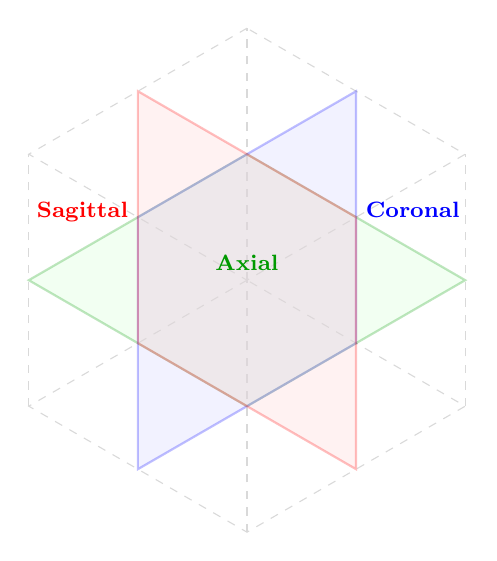
\begin{tikzpicture}[
    scale=1.6, 
    % Manual Isometric Projection:
    x={(-0.866cm,-0.5cm)}, y={(0.866cm,-0.5cm)}, z={(0cm,1cm)},
    plane/.style={opacity=0.25, thick, draw}
]
  % 3D volume cube (Bounding Box)
  \draw[gray!30, dashed] (0,0,0) -- (2,0,0) -- (2,2,0) -- (0,2,0) -- cycle;
  \draw[gray!30, dashed] (0,0,2) -- (2,0,2) -- (2,2,2) -- (0,2,2) -- cycle;
  \draw[gray!30, dashed] (0,0,0) -- (0,0,2) (2,0,0) -- (2,0,2) (2,2,0) -- (2,2,2) (0,2,0) -- (0,2,2);
  
  % Axial Plane (Z = 1) - Green
  \draw[plane, color=green!60!black, fill=green!20] (0,0,1) -- (2,0,1) -- (2,2,1) -- (0,2,1) -- cycle;

  % Coronal Plane (Y = 1) - Blue
  \draw[plane, color=blue, fill=blue!20] (0,1,0) -- (2,1,0) -- (2,1,2) -- (0,1,2) -- cycle;
  
  % Sagittal Plane (X = 1) - Red
  \draw[plane, color=red, fill=red!20] (1,0,0) -- (1,2,0) -- (1,2,2) -- (1,0,2) -- cycle;
  
  % Labels with subtle positioning
  \node[red, font=\bfseries\footnotesize, anchor=north east] at (1,0,1.2) {Sagittal};
  \node[blue, font=\bfseries\footnotesize, anchor=north west] at (0,1,1.2) {Coronal};
  \node[green!60!black, font=\bfseries\footnotesize, anchor=south] at (1,1,1) {Axial};

\end{tikzpicture}
\end{center}

\vspace{-0.2cm}
\begin{columns}[T]
  \begin{column}{0.3\textwidth}
    \centering \textcolor{red}{\textbf{Sagittal}} \\ \scriptsize $x$ = constant \\ (YZ Plane)
  \end{column}
  \begin{column}{0.3\textwidth}
    \centering \textcolor{blue}{\textbf{Coronal}} \\ \scriptsize $y$ = constant \\ (XZ Plane)
  \end{column}
  \begin{column}{0.3\textwidth}
    \centering \textcolor{green!60!black}{\textbf{Axial}} \\ \scriptsize $z$ = constant \\ (XY Plane)
  \end{column}
\end{columns}
\end{frame}

\begin{frame}[fragile]
\frametitle{Extracting Axial Slices}
\begin{lstlisting}
  const out = new Uint8Array(w * h);
  const z = Math.max(0, Math.min(depth - 1, index));
  const offset = z * w * h;
  const range = this.maxValue - this.minValue;

  for (let i = 0; i < w * h; i++) {
    // Linear normalization: [min, max] -> [0, 255]
    const norm = (this.data[offset + i] - this.minValue) / range;
    out[i] = Math.round(norm * 255);
  }
  return { data: out, width: w, height: h };
\end{lstlisting}
\begin{block}{Efficiency}
Axial slices are the fastest to extract because they correspond to a contiguous block of memory in our linear array.
\end{block}
\end{frame}

\begin{frame}[fragile]
\frametitle{Improving Contrast: Windowing}
To see bone or soft tissue specifically, we apply a linear transform based on a \textbf{Center} ($C$) and \textbf{Width} ($W$):

\begin{lstlisting}
const low = center - width / 2;
const high = center + width / 2;

// Inside the loop:
let val = this.data[offset + i];
let normalized = (val - low) / (high - low);
out[i] = Math.max(0, Math.min(255, normalized * 255));
\end{lstlisting}

\begin{table}
\small
\centering
\begin{tabular}{lrr}
\hline
\textbf{Tissue} & \textbf{Center (L)} & \textbf{Width (W)} \\ \hline
Bone            & +400               & 1500               \\
Soft Tissue     & +50                & 400                \\
Lung            & -600               & 1500               \\ \hline
\end{tabular}
\end{table}
\end{frame}

\begin{frame}[fragile]
\frametitle{Extracting Sagittal Slices (X-Plane)}
\begin{lstlisting}
  const out = new Uint8Array(D * H); // z x y
  const x = Math.max(0, Math.min(W - 1, index));
  for (let y = 0; y < H; y++) {
    const yOffset = y * W; // Row offset
    for (let z = 0; z < D; z++) {
      // Manual Indexing: x + yW + zWH
      const volumeIdx = x + yOffset + (z * W * H);
      const voxel = this.data[volumeIdx];
      const outIdx = y * D + z;
      out[outIdx] = ((voxel - min) / range) * 255;
    }
  }
  return { data: out, width: D, height: H };
\end{lstlisting}

\begin{alertblock}{Performance Challenge: Non-Contiguous Access}
Unlike Axial slices, Sagittal voxels are separated by exactly \texttt{width} elements (for $y$) and \texttt{width * height} elements (for $z$). This results in poor \textbf{cache locality}.
\end{alertblock}
\end{frame}

\begin{frame}[fragile]
\frametitle{Extracting Coronal Slices (Y-Plane)}
\begin{lstlisting}
  const out = new Uint8Array(D * W); // z x x
  const y = Math.max(0, Math.min(H - 1, index));
  const yOffset = y * W; // Constant row offset
  for (let x = 0; x < W; x++) {
    for (let z = 0; z < D; z++) {
      // Indexing: x + (y-const) + z*(W*H)
      const volumeIdx = x + yOffset + (z * W * H);
      const outIdx = x * D + z;
      const voxel = this.data[volumeIdx];
      out[outIdx] = ((voxel - min) / range) * 255;
    }
  }
  return { data: out, width: D, height: W };
\end{lstlisting}

\begin{block}{Memory Access Pattern}
The Coronal plane samples voxels that are exactly $W \cdot H$ units apart in the linear array for each $z$ step.
\end{block}
\end{frame}

\begin{frame}
\frametitle{Slice Extraction Complexity}

\textbf{Time Complexity:}
\begin{itemize}
  \item Axial: $O(W \times H)$ - single plane lookup
  \item Sagittal: $O(W \times D)$ - multiple lookups
  \item Coronal: $O(W \times D)$ - multiple lookups
\end{itemize}

\vspace{0.5cm}

\textbf{Normalization:}
\begin{itemize}
  \item Convert float voxels to 8-bit grayscale
  \item Compute min/max during volume construction
  \item Apply linear mapping:
  $$\text{output} = \frac{\text{voxel} - \text{min}}{\text{max} - \text{min}} \times 255$$
  \item Enables proper visualization of contrast
\end{itemize}
\end{frame}